\documentclass[pdftex,11pt,a4paper]{article}
\usepackage{anysize}
\marginsize{2.5cm}{2.5cm}{1.5cm}{1.5cm}
\usepackage[pdftex]{graphicx}
\usepackage{wrapfig}
\usepackage{url}
\usepackage{listings}
\usepackage{color}
\usepackage{textcomp}

\lstset{
	backgroundcolor=\color{lbcolor},
	tabsize=2,
	language=java,
	numbers=left,
	numbersep=5pt,
        basicstyle=\scriptsize,
        upquote=true,
        aboveskip={1.5\baselineskip},
        columns=fixed,
        showstringspaces=false,
        extendedchars=true,
        breaklines=true,
        prebreak = \raisebox{0ex}[0ex][0ex]{\ensuremath{\hookleftarrow}},
        showtabs=false,
        showspaces=false,
        showstringspaces=false,
        identifierstyle=\ttfamily,
        keywordstyle=\color[rgb]{0,0,1},
        commentstyle=\color[rgb]{0.133,0.545,0.133},
        stringstyle=\color[rgb]{0.627,0.126,0.941},
}



\definecolor{listinggray}{gray}{0.9}
\definecolor{lbcolor}{rgb}{0.9,0.9,0.9}
\linespread{1.2}
\setlength{\parindent}{0pt}
\setlength{\parskip}{1ex plus 0.8ex minus 0.2ex}

\usepackage{fancyhdr}

\pagestyle{fancy}
\lhead{\footnotesize {Systems Architecture Project} }
\rhead{\footnotesize {Client orders framework} }

\renewcommand\headheight{24pt}
\renewcommand\footrulewidth{0.4pt}

\clearpage
\newcommand{\HRule}{\rule{\linewidth}{0.5mm}}

\author{John \textsc{Flanagan} 0702009 \& Marcin \textsc{Wrzeszcz} 0726753 }
\title{TITLE GOES HERE}
\date{\today}

\begin{document}

\begin{titlepage}
 
\begin{center}
 
 
% Upper part of the page
%\includegraphics[width=0.8\textwidth]{images/logo.pdf}\\[3.5cm]
 
%\textsc{\LARGE Ubiquitous Merchant Legerity}\\[1.5cm]
 
\textsc{\LARGE Assignment 1}\\[3.5cm]
 
 
% Title
\HRule \\[0.6cm]
{ \huge \bfseries Retail software framework}\\Concurrent Architecture\\[0.4cm]
 
\HRule \\[4.0cm]
 {\large \today}\\[9.0cm]

\begin{flushleft} \large
\emph{Module:}\\
CS4135 Software Architecture
\\[0.4cm]
\emph{Authors:}\\
Marcin \textsc{Wrzeszcz} 0726753 \& John \textsc{Flanagan} 0702009
\end{flushleft}

 
\vfill
 

 
\end{center}
 
\end{titlepage}


\begin{center}
	Blank marking scheme
\end{center}

\pagebreak

\tableofcontents
\pagebreak

\section{Business scenario}
Our team have been tasked by a large computer manufacturer with the design and implementation of a software framework. They are attempting to automate their processes as well as hoping to sell products to customers online. The driver for their decision to automate  its processes has been predominately the current economic crisis, with them aiming to minimise administration staff with the introduction of this software. 

Like many of the large computer manufacturing corporations they have base products which the home or business user may customise to meet their requirements. The components that these products comprise of must be easily interchangeable. 

In the organisations drive to increase online sales, it is expected that this framework not only support integration with web services but also a number of unique business requirements. For example the framework should support support multiple regions taxes and currencies, composition rules for components and the simple addition of new base configurations and products.

While these requirements above may seem initially quite demanding, they are quite typical of the real world business demands for these types of framework.

\pagebreak
\section{Incorporated design patterns}
\subsection{Abstract factory}
\subsection{Factory method}
\subsection{State pattern}
\subsection{Builder pattern}
\subsection{Composite pattern}
\subsection{Observer pattern}

\pagebreak
\section{Creational design patterns}
In the scope of the framework we have two separate areas where creational design patterns are utilised, the creation of states for managing store locale and the creation of products. Of these the creation of products is the most interesting so we will concentrate on this primarily.

Our design for the generation of products aimed to keep the system as generic as possible, enabling developers to easily swap the ‘computer’ package with that of one which creates cars for example. With this requirement much consideration was given to its design and hierarchy. After much research and discussion we decided to use the abstract factory pattern in conjunction with the builder pattern. This enabled us to build factories for different products and for each factory control the assembly of each type of product.

Below is an simplification of our creational structure, in the outermost factory package only the most generic structures were defined, the ‘AbstractFactory’ and the ‘Product’ interface. Within the factory package a further package is created for category of product in this example these are the computer and printer packages.

\begin{center}
	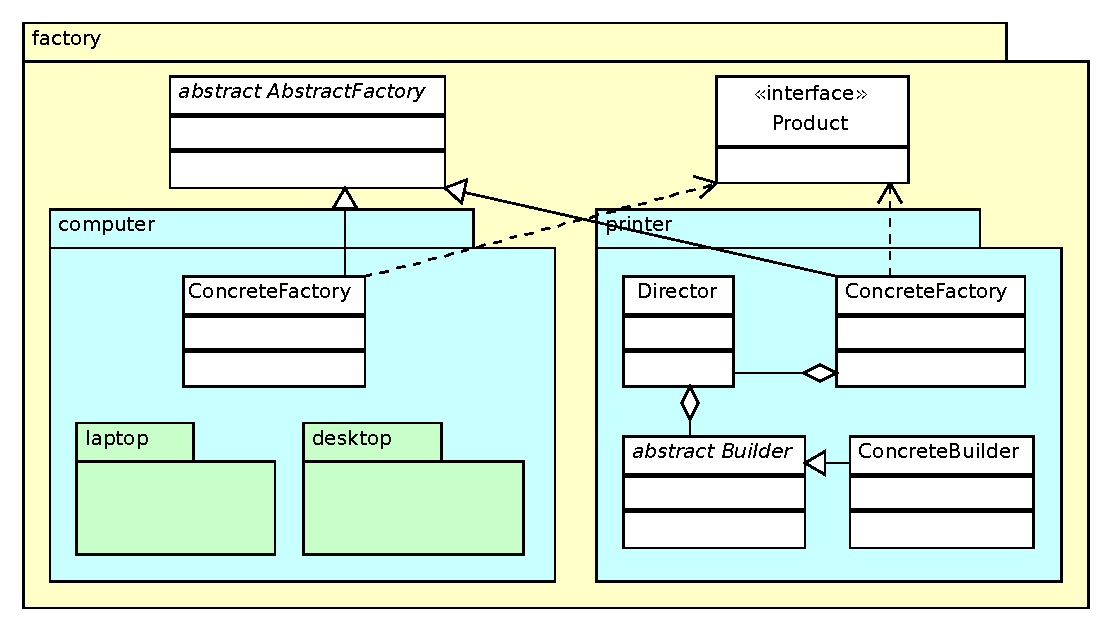
\includegraphics[scale=0.75]{images/creational_diagram.pdf}
\end{center}

This structure offered us the great flexibility in the creation of different product types, while maintaining ‘rules’ for the generation of each product type thanks to the inclusion of the builder pattern.

\subsection{Abstract factory}

To construct an implementation of the AbstractProductFactory you must pass the super type a reference to an observer, this enables us to register the \emph{OrderManager} as a observer of all products created. Which we in-turn use to notify the \emph{OrderManager} when a product is modified.

We designed the abstract factory to only have only one public interface \emph{createProduct(ProductsEnum)} which takes a \emph{ProductsEnum}. As ilustrated in the code fragment \emph{createProduct(ProductsEnum)} uses a switch statement to redirect the program flow to the relevant private method \emph{createGamingDesktopComputer()}. From these private methods we then instantiate a \emph{ComputerBuilder} which is really a director from the builder pattern and populate it with a \emph{ConcreteBuilder}.

This scheme enables us to in time add products of many types to the framework, while maintaining a level or rigidity among the product family's.

\lstinputlisting{code/abstractfactory.java}

\subsection{Builder pattern}

!!!!!how the builder works

\subsection{Observer in creation}
As previously mentioned when instantiating a factory we must pass a ‘OrderManager’ reference, we store this reference and on creation of a new product we register the ‘OrderManager’ as being an observer. This enables the order manager to perform a price recalculation every time a leaf is modified in the composite.

Although this implementation is not designed with performance in mind, as any time a composite is updated with a leaf we must rescan all products for a price change. This solution does offer a clean and structured way for ensuring we keep the cached price up-to-date in the \emph{OrderManager}.

\pagebreak

\section{Unit testing}

To create a reliable framework it is important to have good test coverage of the code, to ensure correctness firstly and secondly to help stop regressions being introduced to the framework. We chose to follow the Test-Driven Development paradigm, as it was a good indicator or development progress and also helped ensure a level of quality. This was largely a successful endeavour although on occasion it was easy to just continue working on the class without any test coverage and absolutely helped to drive the progress of development.

Our unit tests were created using the \emph{JUnit} testing framework\cite{website:junit}, the most common for the \emph{Java} platform. We found this to be quite easy to get up and running and the writing of tests was quite trivial.

\lstinputlisting{code/unittest.java}

In the above code sample, we have included an example of the type of test we are running against the framework. This particular test, performs a series of basic actions including adding a product and decorating a number of components. At the end we test that the price has increased, this test could be enhanced by calculating the extra price and ensuring the new price is equal to the old price plus the added components price.

Each of our tests contain a number of assertions, with any of which failing the overall test will fail. Outside of these individual tests we also use the \emph{setup()} method (not ilustrated here) to create a new instance of the \emph{OrderManager} for each test to ensure the preconditions are met.
\pagebreak

\section{new}
\subsection{Problems encountered and their solutions}
\subsection{Computer Factory}
During the design phase team decided that ComputerFactory class is going to contain following classes: createLowComputer(), createMidComputer(), createHighComputer() and similar for creating laptop products. However every time new produc would be added or old product would be changed it would require so major code rewrites in client implementation. That is why it was decided to implement class createComputer(Enum type) that would be responsible for creating a new instance of any computer (it contains : createLowComputer(), createMidComputer() and so on methods). Now client doesn't have to call each method separately instead it calls the same function with different parameter. This solution created a level of abstraction between client and factories and made code more reusable.

\subsection{Scalability and Reusability}
There are several cases in the UML diagram produced by the team of interfaces that look redundant (ComponentInterface, DecoratorInterface). They are either empty or are realised only by another interface. However this was done on purpose to employ idea of reusability and scalability. Decorator interface might serve as interface to any produc it is not tied to computer products only. So if in future a company decides to increase range of products that they distribute it would be easier for team to realise DecoratorInterface, rather then refractor the code to support new range of products. 

\subsection{Code Selection}
Team found out that usage of strings as parameter for selecting products would be problematic and could create hard to read and hard to maintain code. Adding or removing product would be time consuming. The solution that team came up with was found to solve all problems - the usage of enumerations. Enumerations were used instead of strings for any method that was taking an parameter that was used as a way of selecting specific code, for example calculateTax (Enum region) would execute only code responsible for calculating tax in particular region. This proved to be a very effective and robust way to deal with selection of code; furthermore switch case could be utilised with great readability improvement:


\begin{lstlisting}
switch(computerType){
case COMPUTER_GAMING: code_block_1; break;	
case COMPUTER_OFFICE: code_block_2; break;
case COMPUTER_LAPTOP: code_block_3; break;
}

Instead of:
	
if (computerType == "gamingComputer") {
		code_block_1;
}else if(computerType == "homeComputer") {
		code_block_2;
}else if(computerType == "laptop") {
		code_block_3;
}else{
	else_code_block;
}
\end{lstlisting}

\pagebreak

\section{Criticism and Improvements}
\subsection{Observer}
ComputerComposite is using observer whenever a change in composite occur i.e. new object is added,  removed or decorated. Every time this happens notifyObserver() is invoked. Team's implementation of the observer does not describe the nature of change that occured but only points to object that just changed.An improvement could be employed here, method notifyObserver() could return a reference to leaf back to observer. By using this improvement an observer could update its data via methods call on leaf object. For example when user issues removal of RAM, the RAM leaf object would be dereferenced from its composite parent. Then the reference would be used by orderManager ( RAM.getPrice() ) to update the totalPrice value.
Currently orderManager is notified that the state of "computerProduct" has been altered, so it request getPrice() on root element of "computerProduct" and then it will execute this method on every node in tree to get totalPrice.
If there is a lot of changes to "computerProduct" then system would have to issue the getPrice() on it. This leads to costly and frequent reqursive calculation of total price. With improved implementation of the observer the orderManager object needs to add/subtrack price value of received leaf from the total price.

\subsection{Composite Pattern: safe vs transparent}
Composite contains two lists, one for storing references to all composite children and second list for storing all leaves. If parent of composite class executes getChildern(), composite class have to create a new list that contains "composites" and "leaves".
If getChildern() call was to be executed repetevly then it might be a better idea to create a third list that contains other two lists. The overhead would be minimal as third list contais of references to already existing objects.
This is safe approach to design of the composite pattern as leves do not have access to the same methods as parent. It was found that it would be easier to use transparent approach while designing composite. Transparent approach treats composite and leaf as the same object but leaf does not perform composite methods instead it contais stubs for those methods.

\subsection{UML workbench}
Because of the UML workbench used by team that does not support the generation of class diagrams from the code the synchronisation og the UML model with the code would be too time consuming for the purpose of this project. Therfore at the stage in the project we were happy that we met the design pattern requirements. We used workbench to automaticaly generate the clasess and we chose not to keep model and the code in synch.

\subsection{Decorator}

Team discovered that implementation of the decorator patter could be achieved via two approaches. Wrapping the whole computer object with a decorator for example additional RAM, or particular composite object were to be wrapped with decorator i.e. RAM was wrapped with extra RAM. Even though the first approach was quickly decided to be easier approach it was found that it would decrease computer object flexibility after it was wrapped with additional decorators. Team decided that implementing decorators for each composite component would make code considerably more maintainable. Also accessing information about particular composite object through the computer object would be much easier to implement as there will not be any super class above computer that computer would have to know of.

\pagebreak

\section{UML Diagrams}

\pagebreak

\section{Deployment considerations}
Due to the inherently generic nature of the framework it is possible to be deployed on a number of infrastructures. As proof of concept we built both a traditional GUI application and a Representational State Transfer (RESTful)\cite{REST} implementation to utilise the framework. Representing the traditional and more modern sides of client/server architecture.

\subsection{Desktop application}

\subsection{Webservice}

Web-services are a popular mechanism for exposing a software's functionally over HTTP with a high degree of system and language interoperability. These services can be broadly categorised into RPC and Resource based.

RPC (remote procedure call) is a tried and tested mechanism, and is conceptually an extension to a regular or local procedure call. But due to this constraint of exposing a specific function, these mechanisms tended to be quite system and language dependant. In 2000 Roy Fielding presented his doctoral dissertation where he described "Representational State Transfer"\cite{REST} which described a mechanism modeled around the standard HTTP (GET, POST, UPDATE, DELETE) operations and were resource orientated (giving each entity a unique URI) as opposed to the RPC stored state paradigm. RESTful services have be steadily gaining momentum, and due to this popularity and language/system abstraction, we chose to create a RESTful web-service as a proof of concept for the framework.

\subsubsection{Vendor offerings}
Because of the simplicity of the REST concept, which is based on HTTP which has only four operations as mentioned earlier. There are frameworks for creating RESTful applications for almost every conceivable language, from Clojure\cite{website:compojure-rest} to Javascript\cite{website:persevere}. It is common for developers to use a REST framework that runs within a Application Server such as Tomcat\cite{website:tomcat} or JBoss\cite{website:jboss}. But due to the lightweight nature of the paradigm we were keen on not running the service on a heavy weight application server.

A number of light weight REST frameworks for Java exist, below are a list of the more popular offerings.

\begin{enumerate}
	\item[JAX-RS] A Java JCP spec for RESTful webservices utilising Java Annotations. A number of implementations of the specification exist Apache CXF, Jersey, RESTEasy and Restlet.
	\item[Zipwire-REST] A framework based on the ActiveResource pattern which enables Java object to be manipulated through REST, is a lightweight manner.
	\item[SerfJ]
\end{enumerate}

\subsubsection{Restlet}
Restlet was chosen for this development as it seemed to be the most modern of the feature complete and lightweight frameworks. Restlet also conforms to the JAX-RS JCP specification\cite{website:jax-rs_jcp} making the knowledge gained from this endeavour more valuable.

This library is available under a number of different licences including CDDL ver 1.0, LGPL ver 2.1, LGPL ver 3.0 and EPL ver 1.0. Some larger companies may have difficulty with these licences due to the lack of freedom licences like BSD or Apache offer.

The popularity of this framework is evident in the number of maintained ports for platforms such as Google Web Toolkit, Google App Engine and Android as well as versions for both Java EE and Java SE.

\subsubsection{Development issues}

\subsubsubsection{JSON or XML}

\subsubsubsection{Object serialization}

\subsubsubsection{Web browser security model}

\subsubsection{Deployment diagram}


\pagebreak


\def\refname{}
\bibliography{references}
\bibliographystyle{plain}

\end{document}
